\begin{graphicspathcontext}{{./chapters/sarl/imgs/},{./chapters/sarl/imgs/auto/},\old}

\begin{frame}[t]{Agents Do Not Talk Directly}
	\begin{block}{Key Principle}
		\emph{Agents never interact directly} with each other. \\
		All interactions pass through a shared \emph{interaction medium} called a \emph{Space}
	\end{block}
	\begin{columns}
		\begin{column}[t]{.5\linewidth}
			\smaller
			\Emph{Without SARL model:} \\
			\begin{itemize}
			\item Agent~A calls Agent~B directly
			\item Tight coupling
			\item Hard to control who hears what
			\end{itemize}
		\end{column}
		\begin{column}[t]{.5\linewidth}
			\smaller
			\Emph{With SARL model:} \\
			\begin{itemize}
			\item Agent~A emits an \emph{event} into a \emph{space}
			\item Agent~B is a \emph{participant} of the space and receives the event
			\item Loose coupling; fully decoupled
			\end{itemize}
		\end{column}
	\end{columns}
	\begin{center}
		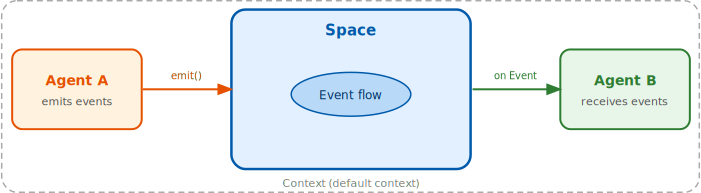
\includegraphics[width=.8\linewidth]{sarl_interactions}
	\end{center}
\end{frame}

\begin{frame}[t,fragile]{Event: The Unit of Interaction}
	\begin{block}{Definition}
		An \emph{event} is the \emph{elementary unit of interaction} inside an event space. \\
		It represents \emph{some occurrence} that may trigger a reaction in a listener
	\end{block}
	\smaller
	\begin{columns}
		\begin{column}[t]{.5\linewidth}
			\Emph{Declaring an event:}
			\begin{sarllisting}[basicstyle=\tiny]
event MyEvent {
	val message : String
	val index   : int
}
			\end{sarllisting}
			\vspace{-.5cm}
			\Emph{Key points:}
			\begin{itemize}
			\item An event carries \emph{data} (fields)
			\item Fields declared with \code{val} are read-only
			\item Events can inherit from other events
			\item Every event has a \emph{source} address (set automatically)
			\end{itemize}
		\end{column}
		\begin{column}[t]{.5\linewidth}
			\Emph{Receiving an event in an agent:}
			\begin{sarllisting}[basicstyle=\tiny]
agent MyAgent {
	uses Logging
	on MyEvent {
		// "occurrence" refers
		// to the received event
		info(occurrence.message)
	}
}
			\end{sarllisting}
			\vspace{-.5cm}
			\textbf{Emitting an event:}
			\begin{sarllisting}[basicstyle=\tiny]
agent MyAgent {
	uses DefaultContextInteractions
	def run {
		emit(new MyEvent("hi", 1))
	}
}
			\end{sarllisting}
		\end{column}
	\end{columns}
\end{frame}

\begin{frame}[fragile]{Event Hierarchy}
	\begin{block}{Events can extend other events}
		SARL events form a class hierarchy, just like Java/Xtend classes
	\end{block}
	\begin{sarllisting}[basicstyle=\scriptsize]
event BaseEvent {
	val id : int
}
event SpecialEvent extends BaseEvent {
	val extra : String
}
	\end{sarllisting}
	\vspace{-1cm}
	\begin{columns}
		\begin{column}[t]{.5\linewidth}
			\begin{description}
			\item A handler declared with \code{on BaseEvent} also fires for \code{SpecialEvent}
			\item[Built-in events] \code{Initialize}, \code{Destroy}, \code{AgentSpawned}...
			\end{description}
		\end{column}
		\begin{column}[t]{.5\linewidth}
			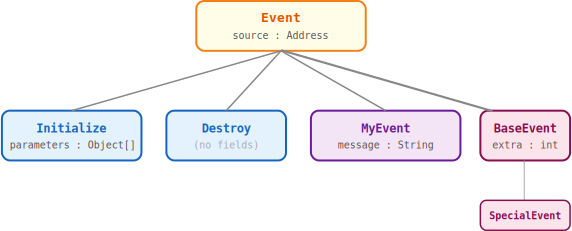
\includegraphics{sarl_event_hierarchy}
		\end{column}
	\end{columns}
\end{frame}

\begin{frame}{Space: the interaction medium}
	\begin{definitionblock}{Space}
	Space is the \emph{support} of interaction between agents, following the rules defined by its \emph{space specification}
	\end{definitionblock}
	\vspace{.5cm}
	\begin{columns}
		\begin{column}[t]{.5\linewidth}
			\Emph{Properties:}
			\begin{itemize}
			\item Identified by a unique \code{SpaceID}
			\item Contains \emph{participants} (agents)
			\item Two kinds of participant:
				\begin{description}
				\item[Strong] space is alive as long as one strong participant is present
				\item[Weak] space can be destroyed if only weak participants remain
				\end{description}
			\end{itemize}
		\end{column}
		\begin{column}[t]{.5\linewidth}
			\Emph{Key interface (simplified):}
			\begin{itemize}
			\item \code{getSpaceID()} $\to$ \code{SpaceID}
			\item \code{getNumberOfStrongParticipants()}
			\item \code{isPseudoEmpty()}
			\end{itemize}
		\end{column}
	\end{columns}
\end{frame}

\begin{frame}[t]{Event Space}
	\begin{definitionblock}{EventSpace (built-in space type)}
		SARL natively defines \code{EventSpace}, a space where agents communicate by \emph{emitting and receiving events}
	\end{definitionblock}
	\vspace{.25cm}
	\smaller
	\begin{columns}
		\begin{column}{.4\linewidth}
			\Emph{Key operations:}
			\begin{compactitemize}
			\item \code{emit(source, event)} \\
				broadcast to all
			\item \code{emit(source, event, scope)} \\
				send only to agents matching a \emph{scope}
			\item \code{getAddress(agentID)} \\
				retrieve the address of a participant
			\end{compactitemize}
			\Emph{Scope:}
			\begin{compactitemize}
			\item Predicate (filter) that selects the recipients of an event e.g., \code{Scopes.addresses(adr1, adr2)}
			\end{compactitemize}
		\end{column}
		\begin{column}{.6\linewidth}
			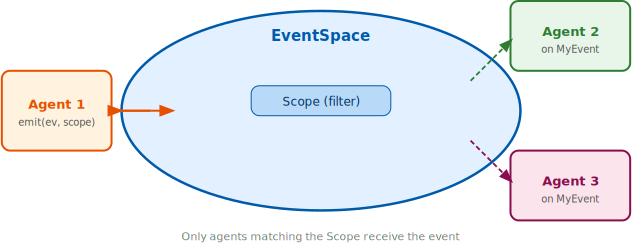
\includegraphics{sarl_event_space}
		\end{column}
	\end{columns}
\end{frame}

\begin{frame}[fragile]{{Space Specification:} Rules of a Space}
	\smaller
	\begin{definitionblock}{Space Specification}
		Defines the \emph{rules} (actions, perceptions, constraints) that govern the interaction within the spaces it creates
	\end{definitionblock}
	\begin{columns}
		\begin{column}[t]{.5\linewidth}
			\Emph{Role:}
			\begin{itemize}
			\item Acts as a \emph{factory}: creates space instances
			\item Encodes the interaction model (who can send, who can receive...)
			\item Determines the \emph{type} of space produced
			\end{itemize}
			\vspace{0.5em}
			\Emph{Built-in Specifications:}
			\begin{itemize}
			\item \code{EventSpaceSpecification} -- basic event space
			\item \code{OpenEventSpaceSpecification} -- agents freely join/leave
			\end{itemize}
		\end{column}
		\begin{column}[t]{.5\linewidth}
			\Emph{Custom specification example:}
			\begin{sarllisting}[basicstyle=\footnotesize]
class MySpaceSpec
      implements
      SpaceSpecification
               <MySpace> {
	def create(id : SpaceID,
	           params : Object*)
	    : MySpace {
		new MySpace(id)
	}
}
			\end{sarllisting}
		\end{column}
	\end{columns}
\end{frame}

\begin{frame}[fragile]{Using a Custom Space in an Agent}
	\begin{sarllisting}[basicstyle=\tiny]
agent MyAgent {
	uses DefaultContextInteractions
	uses Behaviors
	uses Logging

	var mySpace : OpenEventSpace

	on Initialize {
		// Retrieve (or create) a space matching the given spec
		mySpace = defaultContext.getOrCreateSpaceWithSpec(
				typeof(OpenEventSpaceSpecification),
				occurrence.parameters.get(0) as UUID)

		// Register this agent as a strong participant
		mySpace.registerStrongParticipant(asEventListener())
	}

	on MyEvent {
		// Handle the event received from mySpace
		info("Received: " + occurrence.message)
	}
}
\end{sarllisting}
\end{frame}

\begin{frame}{Context: A Boundary for Agent Sub-Systems}
	\begin{block}{Definition}
	A \emph{context} (AgentContext) is a \emph{container} that groups a set of spaces and defines the boundary of an agent sub-system
	\end{block}
	\vspace{.25cm}
	\begin{columns}
		\begin{column}[t]{.5\linewidth}
			\Emph{Properties:}
			\begin{itemize}
			\item Has a unique \code{UUID} identifier
			\item Contains \emph{one or more spaces}
			\item Always has a \emph{default space} (an \code{EventSpace})
			\item New spaces can be created inside a context at any time
			\item Each agent belongs to at least one context
			\end{itemize}
		\end{column}
		\begin{column}[t]{.5\linewidth}
			\Emph{Key interface (simplified):}
			\begin{itemize}
			\item \code{getID()} $\to$ \code{UUID}
			\item \code{getDefaultSpace()} $\to$ \code{EventSpace}
			\item \code{getSpaces()} $\to$ all spaces
			\item \code{createSpace(spec, id)}
			\item \code{getOrCreateSpaceWithSpec(spec, id)}
			\end{itemize}
		\end{column}
	\end{columns}
\end{frame}

\begin{frame}{{Default Context} and Default Space}
	\begin{block}{Every agent has a default context}
	When an agent is created, it is placed inside a \textbf{default context}
	with a \textbf{default space} (an \texttt{EventSpace}).\\
	The built-in capacity \texttt{DefaultContextInteractions} provides easy access to both.
	\end{block}
	\begin{center}
		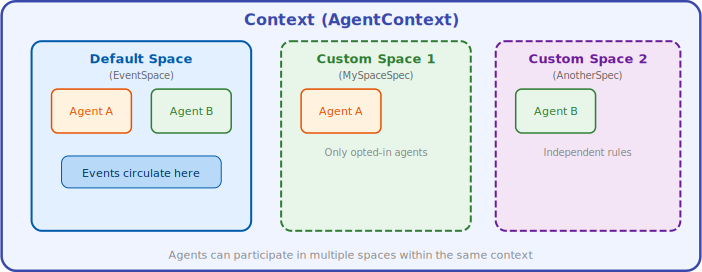
\includegraphics[width=.9\linewidth]{sarl_context_space}
	\end{center}
\end{frame}

\end{graphicspathcontext}

\endinput

